\chapter{Radio electronic characteristics}

By the time the \gls{rf} signal has reached the acoustic transducer, it has
been synthesized from a reference signal, amplified, and matched to the
impedance of the \gls{aod} transducer. We are going to inspect the \gls{rf}
signal characteristics at each transmission and find that each stage
unintentionally carries out frequency dependent amplitude modulation which,
as we will see in the next chapter, is responsible for the complex intensity
distribution observed with the photodiode.

\section{Digital signal synthesizer}

We already covered the fundamental functionality of the \gls{dds} in XX and
its integration in our experimental setup in YY, yet we are missing physical
measurements.

Physical analysis of the \gls{dds} output \gls{rf} signal is in fact no
simple endeavour as usual operation time scales are of many magnitudes
greater than the signal periodicity. The strategy we used to resolve this
circumstance is depcited in \Cref{fig:dds_sweep_window}. The strategy
consists of capturing multiple, small time windows of the signal which
delayed would cover the complete signal trace.

\begin{figure}[h]
  \centering
  \includegraphics[width=\textwidth]{\mediadir{diagram/sweep-window.pdf}}
  \captionsetup{width=.8\textwidth}
  \caption{Idealized \gls{dds} signal output with constant frequency and
    linear ramp over the sweep duration. The measured window only captures
    a subset of the complete sweep but can be delayed to cover the complete
    sweep duration.}
  \label{fig:dds_sweep_window}
\end{figure}

The experimental setup is schematically drawn in
\Cref{fig:dds_sweep_window_setup}. In between the oscilloscope and the
trigger source we inserted a pulse generator. The pulse generator width
corresponds to the delay time of the oscilloscope as the oscilloscope is
configured to capture on the falling edge signal of the pulse generator.

\begin{figure}[h]
  \centering
  \includegraphics[width=\textwidth]{\mediadir{setup/sweep-window.pdf}}
  \captionsetup{width=.8\textwidth}
  \caption{By inserting a pulse generator in between the trigger source and
  the oscilloscope we can delay the capture window of the oscilloscope by
the pulse width.}
  \label{fig:dds_sweep_window_setup}
\end{figure}

In \Cref{tab:dds_signal_parameters} we can find an overview of the
experimental parameters.

\begin{table}[h]
  \centering
  \begin{tabular}{|c|c|c|c|c|}
    \hline
    Start frequency $f_0$ &
    Final frequency $f_1$ &
    Sweep duration $T_s$ &
    Window duration $T_w$ \\
    \hline
    \SI{80}{\mega\hertz} &
    \SI{4.88}{\mega\hertz} &
    \SI{200.00}{\micro\second} &
    \SI{26.84}{\milli\second} \\
    \hline
  \end{tabular}
  \captionsetup{width=.8\textwidth}
  \caption{Experimental parameters used to inspect the output \gls{rf} signal
  of the \gls{dds}.}
  \label{tab:dds_signal_parameters}
\end{table}

The specified frequency range is motivated to cover
the greatest possible spatial dimensions permitted by the dimensions of the
optics. Sweep and window duration where selected as a compromise between the
oscilloscope being able to resolve the signal fine enough to perform
\gls{fft} and the sweep duration being comparable to later experiments. Time
delay between windows was choosen to be $T_s/300$, thus we will capture 300
overlapping time windows.

\subsection{Discrete frequency spectrum}

\begin{figure}[h]
  \centering
  \includegraphics[width=\textwidth]{\figuredir{signal/synthesis/spectrogram.pdf}}
  \captionsetup{width=.8\textwidth}
  \caption{Spectrogram of delayed time windows of the \gls{dds} output signal
    configured to perform a frequency sweep from \SI{80}{\mega\hertz} to
    \SI{120}{\mega\hertz}. For an ideal linear sweep we would expect a linear
    timeline of the frequency, instead we observe a discrete set of
    frequencies which reflects the digital nature of the \gls{dds}.}
  \label{fig:signal_synthesis_spectrogram}
\end{figure}

\subsection{Amplitude frequency response}

\section{Amplifier}

\subsection{Transmission spectrum}

\subsection{Amplitude frequency response}

\section{Acoustic transducer}

\subsection{Reflection spectrum}
